\documentclass[
    floatsintext
]{article}

\usepackage{graphicx}
\usepackage{hyperref}
\usepackage{subcaption}
\usepackage{amsmath}

\hypersetup{colorlinks,urlcolor=blue}
\let \shorttitle \textbf
\begin{document}

\section{Visual Search}

\subsection{Motivation}
\shorttitle{Visual Search}

In optimising our tool positional search, we must determine regions of contact that are likely to be good locations for the objects interaction.
The proposal follows the idea mentioned by \cite{battaglia2013}, in that humans build mental models of objects to allow inference over the physical world.
Human subjects would have an understanding over the geometric constraints of the physical world and of the forces generated by their actions.
For example, subjects performing tool fitting tasks, examine the geometry of objects and stop at likely positions before attempting interaction.  

Tool and object interaction baring high likelihood of success, would satisfy two criteria: 
\begin{enumerate}
\item \textbf{Geometric constraints} of the two objects must be met (i.e. the shapes of the two objects should adequately fit)
\item \textbf{Contact forces} generated must correspond to the intention of the actions executed 
  (i.e. for a lifting action, the human subject would focus on points of interaction that would permit vertical forces to be applied)
\end{enumerate}

The total space of possible solutions can be reduced by these criteria without a physics simulation (akin mental simulations \cite{osiurak2014}).
The potential of likely solutions can be later verified using a physics engine. 

\subsection{Geometric Constraints}
The geometries of the tool and object must be compatible. In other words, either the active or passive object's geometry must fit within the gaps and edges of its counterpart.
Tighter fits, offer better transfer of energy and control over the movement of the passive object. A good fit would therefore require less manipulation effort.
In the paradigm of 4CT \cite{osiurak2014}, the effort constraint may explain user's preference for one geometric solution over another.

It is not necessary for the whole geometry of objects to fit. 
It is sufficient that the tools have the necessary parts to act as affordance and functional basis (end effector\cite{zhu2015}).
If the functional part matches the gaps of the passive object, then the configuration is likely to achieve the desired effect. 

\subsubsection{Shape Description and Matching Techniques}
We consider techniques of shape similarity in matching object parts.
Shape analysis techniques have traditionally been engaged in image processing and robot vision for detecting and tracking objects of similar features.
The last two decades have provided many approaches for this type of problem \cite{loncaric1998,zhang2004,veltkamp2001,robert2012}.
Fundamentally, the challenge lies in detecting similarity even as objects undergo geometric transformations (i.e. rotation, translation, scaling and shearing).     

\cite{zhang2004} classify shape similarity into contour-based and region-based techniques. These are further divided into structural and global approaches.
These are further divided into structural and global approaches.
A comprehensive list and relations can be found in fig. \ref{fig:shape_similarity}. 

\begin{figure}[h]
  \centering
  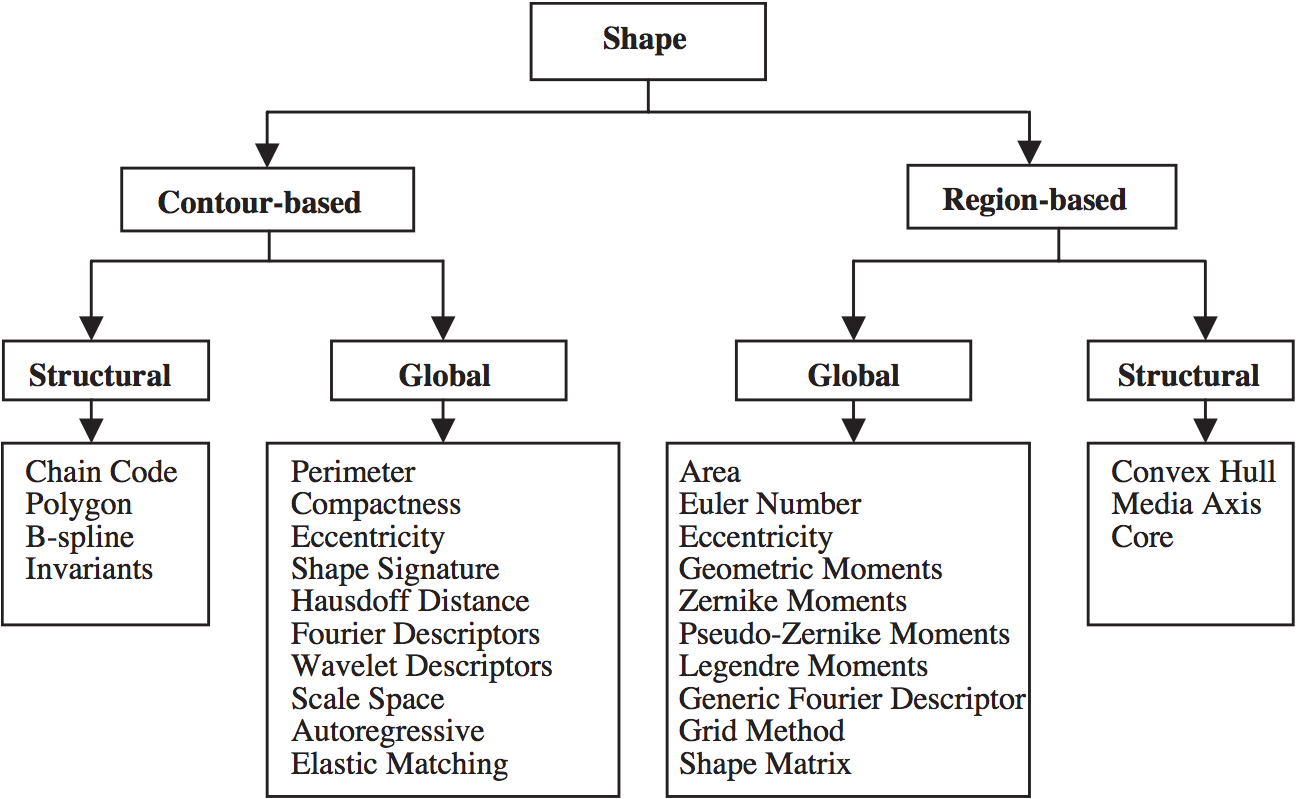
\includegraphics[width=1\textwidth]{./figures/similarity_techniques.png}
  \caption{Classification of shape similarity techniques (reprinted from \cite{zhang2004})}
  \label{fig:shape_similarity}
\end{figure}  

Contour techniques asses shape similarity by extracting features from the edge of detected objects.
In comparison, region techniques work by assessing surface level information such as: colour features, gradient changes and surface medial.
Techniques from both approaches have justification in human perception \cite{chatbri2016}.
Nonetheless, our use case excludes most region-based approaches as tool parts must correspond to shape gaps.
It is hard to consider gaps as having the surface information needed for region-based matching.

In structural approaches, shapes are considered as composed of primitives. In the case of contour techniques, primitives are segments on the boundary of an object.
The organisation of primitives can be linear (feature vector \cite{zhang2004}) or hierarchical (tree like structures\cite{zhu2015}).
Two objects are considered similar when they have the same primitive structures (or features).
In comparison, global approaches make use of shapes as a whole when assessing similarity. 

Both structural and global approaches have justification in human perception \cite{zhang2004}.
Human subjects show a preference for features even when other shape descriptors are available \cite{chatbri2016}.
At the same time, global shape perception seems to precede local feature detection \cite{navon1977}. 

Matching human behaviour requires more insight into human visual perception.
\cite{loncaric1998} describes some theories of human visual perception with interest in image processing.
In a tool use scenario, emphasis should be given to theories describing perception as volumetric, such as through the use of generalised cylinders (known as geons \cite{dickinson2014}).
Such insight may better explain human tool performance, but will however remain for future work.    

\subsubsection{Limitations}
As previously remarked, contour based techniques contain promising approaches for solving tool-object matching problems.
It is important to consider some of the limitations of such techniques, especially with regards to human ability. 

Global contour matching techniques are sensitive to occlusion (i.e. part of the object is hidden from the view point by some obstacle).
In such cases, structural approaches are better suited to identify shapes from visible parts.
Human perception is regarded as able to recognise objects even from sparse information or occluded perspective \cite{loncaric1998}.
In solving tool use scenarios, it is important to consider a subject's visual perspective (point of view).
The geometry of objects may not be fully visible, hiding the functional parts.

Most shape similarity techniques are tailored to analysing image based information (i.e. 2D projections of a 3D space).
Human perception however also makes use of depth related knowledge.
As tool use encompasses real world geometric constraints, any contour based approach would have to adapt to 3D information (e.g. point clouds).
For our scenario, we can simplify the problem of visual analysis by extracting 3D surface point directly from the physics simulator (instead of using 2D projections). 

Additionally, human subjects may attempt tool and object interaction even when parts do not fully match. 
We therefore require a uniform way of assessing the degree of similarity between two contours. 

We next consider a novel and simple approach for assessing object contours.
It avoids most of the problems enumerated above and scales well to multi-dimensional data, whilst also considering human ability.  

\pagebreak[0]
\subsection{Novel Surface Similarity}
Contour matching over two dimensional projections is essentially the problem of assessing the similarity of lines.  
When applied to three dimensional data points the task can be considered as measuring similarity of surfaces.  
The following novel technique can be described as a general approach for assessing surface similarity. 
It is based on principal component analysis (PCA) and Pearson's correlation coefficient. 

\subsubsection{2D Case}
At it's core, the technique assumes that points taken over similar surfaces change value in the same direction and at the same rate. 
For example, consider two lines as in figure \ref{fig:similar_lines_A}. Pairs of points taken from each line change Y axis value at the same time. 
I.e. if point 2 on the red line increases, so does the corresponding point on the blue line.   
More so, compared to figure \ref{fig:similar_lines_B}, the first set of lines change value at the same rate against their Y-axis deviation.
A human observer would assess lines in figure \ref{fig:similar_lines_A} to be more similar than lines in \ref{fig:similar_lines_B},
which are more similar than in figure \ref{fig:similar_lines_C}.

\begin{figure}[h]
  \centering
  \begin{subfigure}{.49\textwidth}
    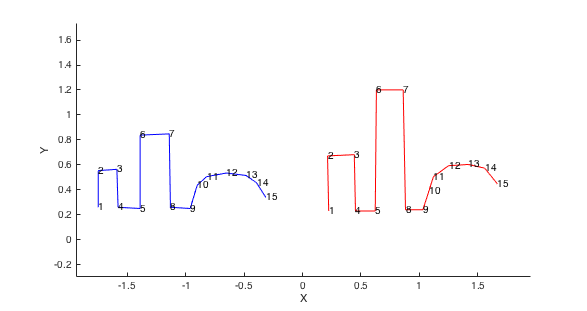
\includegraphics[width=1\linewidth]{./figures/similar_lines_A.png}
    \caption{Same direction \& rate (different scales)}
    \label{fig:similar_lines_A}
  \end{subfigure}
  \begin{subfigure}{.49\textwidth}
    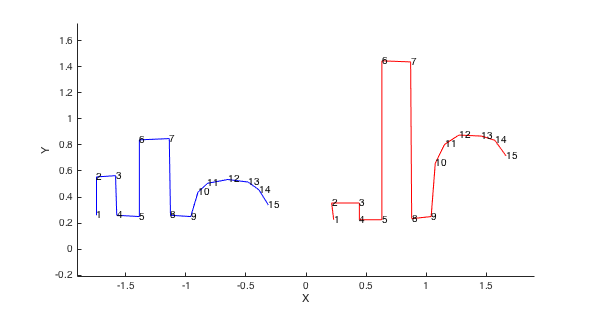
\includegraphics[width=1\linewidth]{./figures/similar_lines_B.png}
    \caption{Same direction but different rates}
    \label{fig:similar_lines_B}
  \end{subfigure}
  \begin{subfigure}{.49\textwidth}
    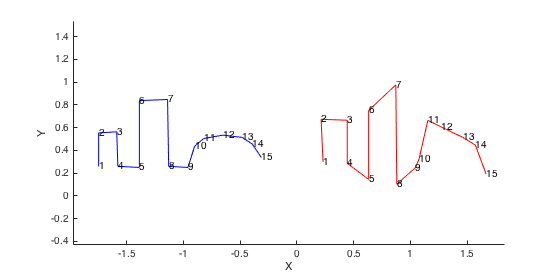
\includegraphics[width=1\linewidth]{./figures/similar_lines_C.png}
    \caption{Different directions}
    \label{fig:similar_lines_C}
  \end{subfigure}
  \caption{Lines of different similarity. From (a) to (c), shown in decreasing similarity.}
\end{figure}

In a scenario where lines share the same orientation (e.g. angle against the X axis), Pearson's correlation provides an adequate measure of line similarity.
The correlation coefficient measures the extent to which two variables ($x_i$ and $x_i^\prime$) 
can be defined through a linear equation ($x_i^\prime = a * x_i + b$). \\

Resulting values are in the range of $[-1,+1]$ where:
\begin{itemize}
    \item values close to +1 represent high similarity
    \item values close to 0 represent dissimilarity 
    \item values close to -1 represent high similarity but mirrored (e.g. points are in reverse order) 
\end{itemize}

Lines with complex curvatures can be expressed through series of points in Cartesian space. 
Affine transformations of scaling\eqref{eq:scale} and translation\eqref{eq:translate} produce new points defining lines who's coordinated are linearly related to the original. 
Pearson's correlation would therefore return high similarity if two lines are linear transformations of each other.    
\begin{equation}
  \begin{bmatrix}
    a_x & 0   & 0   \\
    0   & a_y & 0   \\
    0   & 0   &   1 \\ 
  \end{bmatrix} 
  *
  \begin{bmatrix}
    x_i \\ y_i \\ 1
  \end{bmatrix} 
  = 
  \begin{bmatrix}
    a_x * x_i \\ a_y * y_i \\ 1  
  \end{bmatrix}
  \label{eq:scale}
\end{equation}


\begin{equation}
  \begin{bmatrix}
    1 & 0 & b_x \\
    0 & 1 & b_y \\
    0 & 0 & 1   \\ 
  \end{bmatrix} 
  *
  \begin{bmatrix}
    x_i \\ y_i \\ 1
  \end{bmatrix} 
  = 
  \begin{bmatrix}
    x_i + b_x \\ y_i + b_y \\ 1  
  \end{bmatrix}
  \label{eq:translate}
\end{equation}

In the case of rotation\eqref{eq:rotate} or shearing\eqref{eq:shear}, the linear relationship between points is lost.
A graphical example of the different transformations can be seen in figure \ref{fig:affine_transform}.

\begin{figure}[h]
  \centering
  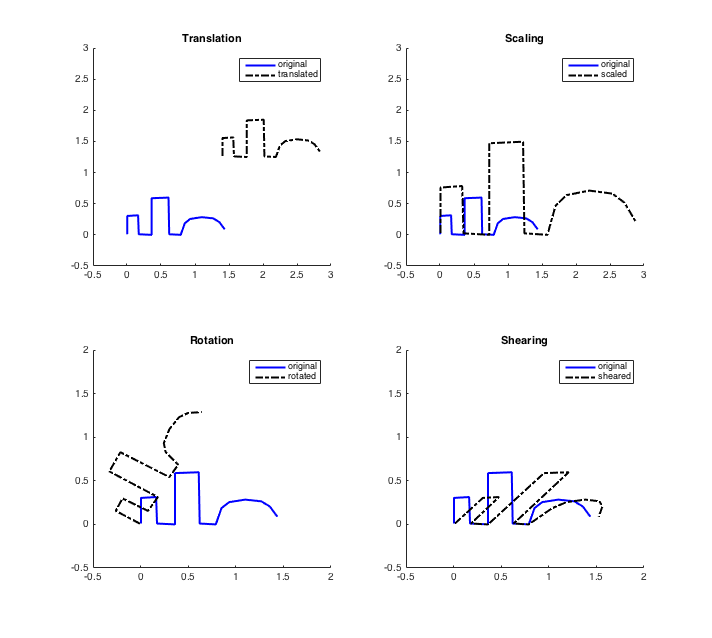
\includegraphics[width=1\textwidth]{./figures/affine_transform.png}
  \caption{Graphical examples of affine transformations}
  \label{fig:affine_transform}
\end{figure}  

\begin{equation}
  \begin{bmatrix}
    cos(\theta)  & -sin(\theta) &   0 \\
    -sin(\theta) & cost(\theta) &   0 \\
    	0   	 &	0       &   1 \\ 
  \end{bmatrix} 
  *
  \begin{bmatrix}
    x_i \\ y_i \\ 1
  \end{bmatrix} 
  = 
  \begin{bmatrix}
    x_i * cos(\theta) - y_i * sin(\theta) \\ x_i * sin(\theta) + y_i * cos(\theta) \\ 1
  \end{bmatrix} 
  \label{eq:rotate}
\end{equation}


\begin{equation}
  \begin{bmatrix}
    1 & h & 0 \\
    0 & 1 & 0 \\
    0 & 0 & 1   \\ 
  \end{bmatrix} 
  *
  \begin{bmatrix}
    x_i \\ y_i \\ 1
  \end{bmatrix} 
  = 
  \begin{bmatrix}
    x_i + h * y_i \\ y_i \\ 1  
  \end{bmatrix}
  \label{eq:shear}
\end{equation}

In a tool use scenario involving rigid bodies, shearing is not a reasonable transformation. Rotation on the other hand is. 
PCA returns a set of unit vectors that indicate the direction in which data has most variation. 
The rotation angle of a line can be removed by aligning the shape's principal components to the main X-Y axis.    
As affine rotations preserve variation, the principal vectors rotate by the same angles that a figure is rotated (figure \ref{fig:pca_rotation}).  

\begin{figure}[h]
  \centering
  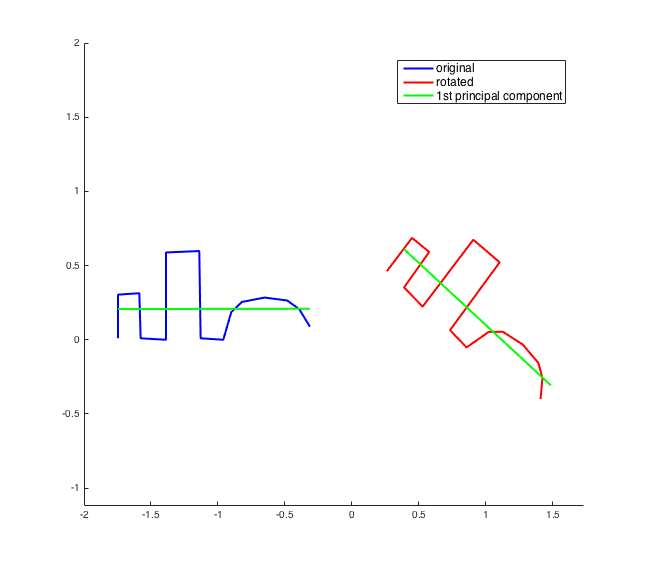
\includegraphics[width=.5\textwidth]{./figures/pca_rotation.png}
  \caption{First principal component rotating with the figure}
  \label{fig:pca_rotation}
\end{figure}  

The principal components of a set of data are orthogonal. 
For that reason, in the case of 2D data points, it is sufficient to align just the first principal component to the X axis.
Even in higher dimensionality of $n$ components, it is sufficient to align the first $n-1$ components.

The rotation angle can be retrieved from:
\begin{equation*}
\alpha = atan2(v_y,v_x)\ mod\ 2\pi 
\end{equation*}
Where $V=(v_x,v_y)$ is the first PCA vector.

After angle retrieval, all points defining a figure are rotated against their mean, in order to perform correlation. 
Similarity is calculated as the product of correlations for the individual X-Y coordinates.
Figures \ref{fig:correlation_2D} and \ref{fig:no_correlation_2D}, demonstrate the approach working on two hand drawn lines. 
Higher correlation is achieved for the more similar lines. 

\begin{figure}[h]
  \centering
  \begin{subfigure}{.5\textwidth}
    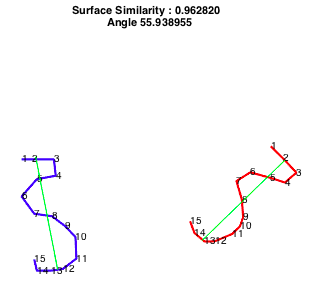
\includegraphics[width=1\linewidth]{./figures/correlation_2D.png}
    \caption{Similar contours}
    \label{fig:correlation_2D}
  \end{subfigure}
  \begin{subfigure}{.44\textwidth}
    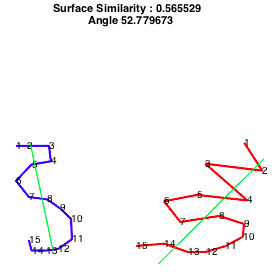
\includegraphics[width=1\linewidth]{./figures/no_correlation_2D.png}
    \caption{Dissimilar contours}
    \label{fig:no_correlation_2D}
  \end{subfigure}
  \caption{Comparison of simalirty measure}
\end{figure}

\pagebreak[2]
\subsubsection{3D case}

The components of the approach allow it to be applied to pairs of surfaces instead of lines. 
As with 2D shapes, points in 3D Cartesian space (i.e. X-Y-Z coordinates) can be organised in a grid structure defining a surface mesh (fig. \ref{fig:mesh_example}).

\begin{figure}[h]
  \centering
  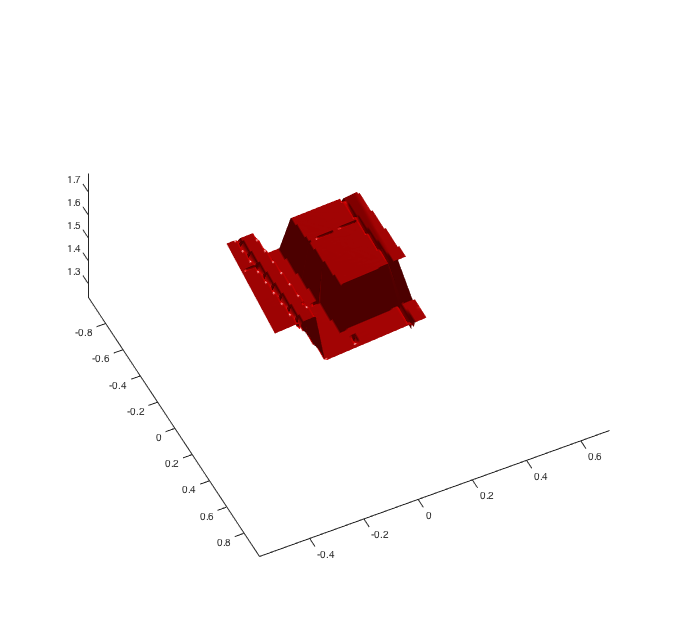
\includegraphics[width=.5\textwidth]{./figures/mesh_example.png}
  \caption{Example of surface mesh}
  \label{fig:mesh_example}
\end{figure}  

The similarity algorithm steps remain the same: 
\begin{enumerate}
    \item Calculate the PCA vectors of the points defining each surface 
    \item Establish the rotation angles for aligning the first two principal vectors of each surface 
    \item Rotate all point of a figure against the mean location, using the established angles
    \item Calculate the product of correlations over all dimensions (i.e. X-Y-Z) 
\end{enumerate}

For 3D space however, calculating angles and applying rotations involve different calculations.
Two angles are required for aligning the first principal component against the X axis: 
\begin{equation*}
  \begin{split}
    \alpha = atan2(v_y^1,v_x^1)\ mod\ 2\pi\\
    \beta = -asin(v_z^1)\ mod\ 2\pi
  \end{split}
\end{equation*}
Where $v^1=(v_x^1,v_y^1,v_z^1)$ is the direction vector of the first principal component.
The second principal component vector must be rotated by $\alpha$ and $\beta$ in order to extract a third angle: 
\begin{equation*}
  \begin{split}
    v^2 = rotY(-\beta) * rotZ(-\alpha) * v^2\\
    \gamma = atan2(v_z^2,v_y^2)\ mod\ 2\pi 
  \end{split}
\end{equation*}
Where $v^2=(v_x^2,v_y^2,v_z^2)$ is the direction vector of the second principal component. 
$rotY(-\beta)$ and $rotZ(-\alpha)$ are rotation matrices taking points counter clockwise around the Y and Z axis.   

Surface points can then be aligned to the primary axes by multiplying them to the corresponding rotation matrices:  
\begin{equation*}
   P = rotX(-\gamma) * rotY(-\beta) * rotZ(-\alpha) * P
\end{equation*}
Where P is the set of points defining the surface mesh.

\subsubsection{Discussion}
The nature of the technique, permits extracting the angle difference between two shapes.  
\end{document}


